\section{Methodology}
Overall the methods examined in this thesis can be divided into two parts; namely those trying to decompose the input into a NN, and those decomposing the weights of a pre-trained NN with subsequent fine-tuning. In the following the methods used within each of these parts will be discussed in detail. All decomposition estimation will be executed using the Python library \textit{TensorLy}\cite{tensorly}, which provides an API for tensor methods using different back-ends\footnote{The back-end is the Python library that is responsible for the low-level calculation and specification of the tensors. Typically \textit{NumPy}\cite{numpy} or \textit{PyTorch}\cite{pytorch}} for calculations. The algorithms for estimating the decompositions will be given in appendix. 

\subsection{Decomposing the Input}
In reality, tampering with the data that is going to be learned is data preprocessing, hence decomposing the input is just a form of this. Data preprocessing is a vital part of almost all ML, because structured data of high quality is simply much easier to learn and to work with. Put in another way: "Garbage in, garbage out". In addition knowledge of the structure and the variance of the data often ease the algorithm development process. The decomposition algorithms seems appropriate for this task due to their ability to exploit the structure of the data. 

The Tucker decomposition is believed to be suitable for data compression tasks \cite{Mørup2011}, hence it seems natural to apply this method to the data before feeding it into and training the NN. The purpose is to let the decomposition do some of the learning beforehand, by exploiting the variance in the data. The Tucker-decomposition is very flexible because it allows for decomposition of only a subset of the dimensions\footnote{This is also called a \textit{partial} Tucker decomposition}, and because it allows for specification of ranks for each dimension individually. Since the ranks correspond to the degree of flexibility, it is easy to choose how flexible the decomposition should be along each dimension. The rank would increase with the level of desired detail along the dimension. This means that if the desire of the algorithm is to differentiate a small set of features, the rank would also be kept small along the relevant dimension.

Since the observations in each the given data sets can be stacked to form a 4 (MNIST) or 5 (THETIS) dimensional tensor, it is fairly straight forward to apply the Tucker decomposition. For $N$ MNIST observations, the stacked tensor $\tensor{X}$ of size $(N \times 1 \times 28 \times 28)$ will be reshaped to $(N\times 28 \times 28)$ due to the single input channel. The decomposition of the now 3rd order tensor becomes:
\begin{equation}
    \tensor{X}^{N\times 28 \times 28} \approx \tensor{G}^{L\times J \times K} \times_1 \bs{A}^{N\times L} \times_2 \bs{B}^{28 \times J} \times_3 \bs{C}^{28 \times K}
\end{equation}
Where $L, J$ and $K$ corresponds to the ranks in each of the dimensions. Here $\tensor{G}$ is the core of the decomposition, $\bs{A}$ corresponds to the loading matrix along the dimension holding the different observations, while $\bs{B}$ and $\bs{C}$ correspond to the loading matrices in the spatial dimensions.

\subsubsection{Example with MNIST 3s and 4s}
Only the observations depicting either a 3 or a 4 will be considered in this example. These digits are chosen due to their distinct shapes, hence ease of classification. Since the purpose is to make the algorithm find the differences between the two different digits, the spatial dimensions will not be decomposed. This means that a so-called partial Tucker-decomposition will be conducted, hence $\bs{B}$ and $\bs{C}$ will be identity matrices. Now experimentally setting the rank to 2, the decomposition of $N$ stacked 3s and 4s becomes:
\begin{equation}
    \tensor{X}^{N\times 28\times 28} \approx \tensor{G}^{2 \times 28 \times 28} \times_1 \bs{A}^{N\times 2} \qquad \Leftrightarrow \qquad \bs{X}_{(1)} \approx \bs{A}^{N\times 2} \ \bs{G}^{2 \times 28\cdot 28}_{(1)}
\end{equation}
Where $\bs{A}$ is the loading matrix in the dimension corresponding to different pictures. With the rank equal to 2, $\bs{A}$ holds 2 values per picture that should ideally be separating the two digits that is to be trained. \autoref{fig:decompExample3_4} shows how the decomposition of the first 100 training examples turns out. It seems the decomposition is able how to find the "general 3" and the "general 4", and then simply use the loadings of $\bs{A}$ to specify how much of each it an observation is. XX shows a scatter-plot of the values of $\bs{A}$ colored to show the loadings corresponding to 3s and 4s respectively. It is clear that the clusters can be distinguished even though there is still some overlap. 

\begin{figure}
    \centering
    \begin{subfigure}{0.45\linewidth}
        \centering
        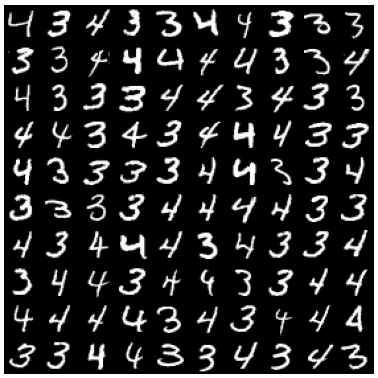
\includegraphics[width=\linewidth]{Pics/05_methodology/3_4_original.png}
        \captionsetup{width=.8\linewidth}
        \caption{Original MNIST training examples including only 3s and 4s.}
    \end{subfigure}
    \begin{subfigure}{0.45\linewidth}
        \centering
        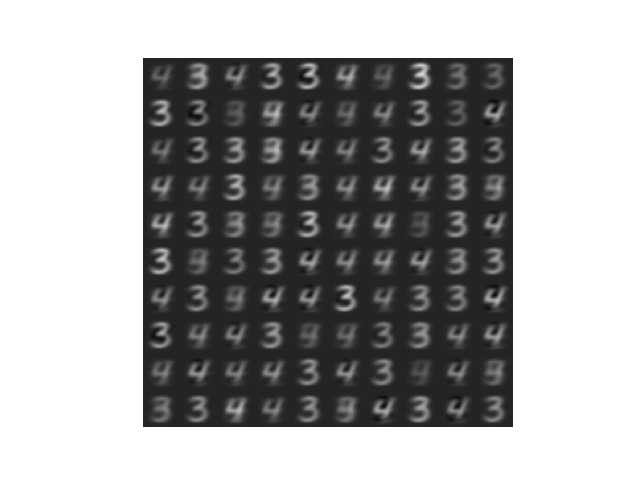
\includegraphics[width=\linewidth]{Pics/05_methodology/3_4_decomp.png}
        \captionsetup{width=.8\linewidth}
        \caption{Decomposed versions of the training examples on the left.}
    \end{subfigure}
    \captionsetup{width=.95\linewidth}
    \caption{MNIST training examples before and after decomposing with only rank 2 in the input dimension. Notice how the decomposed 3s and 4s look more standardized. It seems that every picture is a part standardized 3 and a part standardized 4. }
    \label{fig:decompExample3_4}
\end{figure}

\begin{figure}
    \centering
    \begin{subfigure}{0.99\linewidth}
        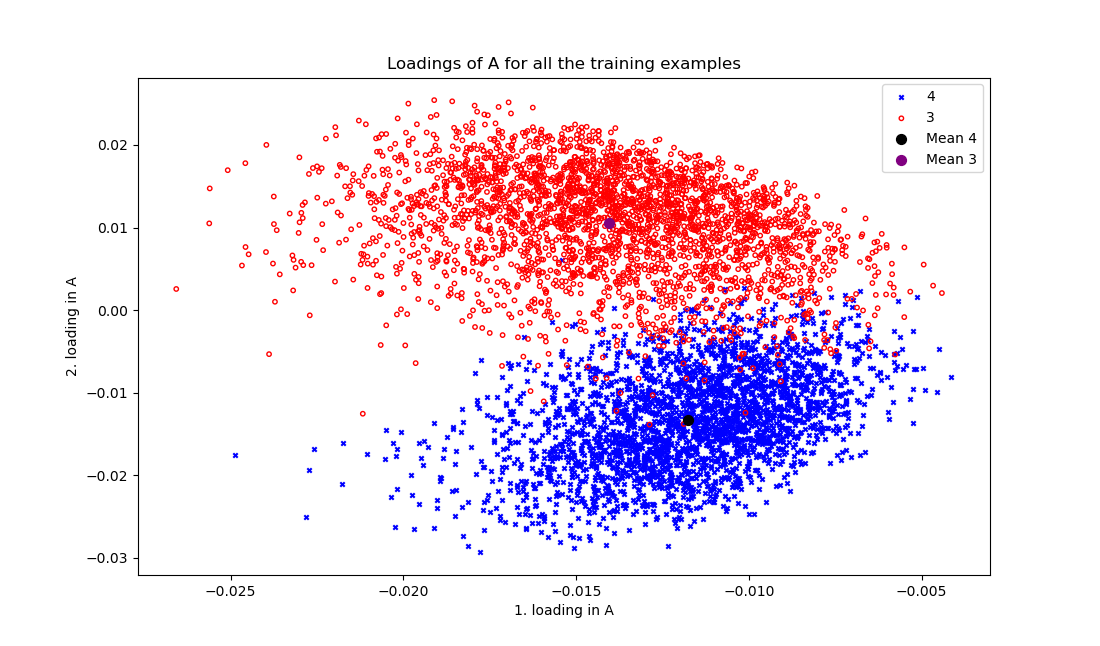
\includegraphics[width=\linewidth]{Pics/05_methodology/LoadingsOfAScatterMNIST.png}
    \end{subfigure}
    \begin{subfigure}{0.3\linewidth}
        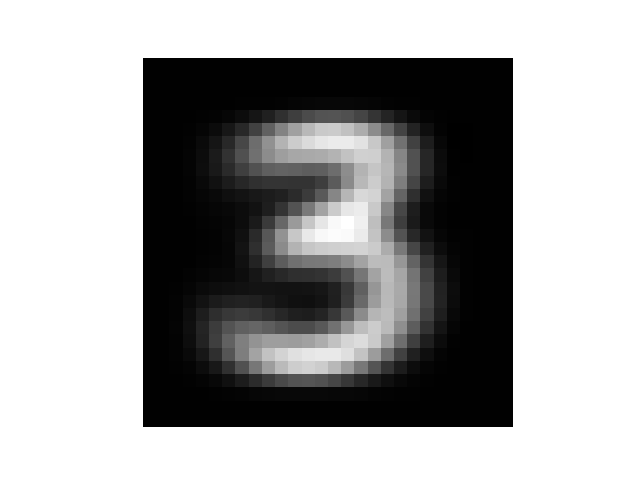
\includegraphics[width=.5\linewidth]{Pics/05_methodology/general3.png}
    \end{subfigure}
    \begin{subfigure}{0.3\linewidth}
        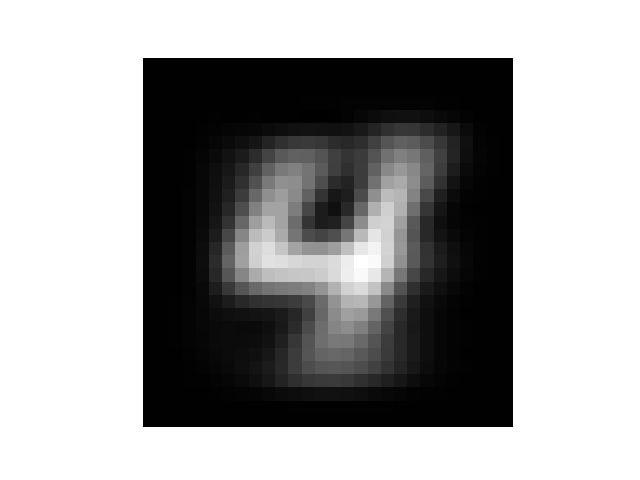
\includegraphics[width=.5\linewidth]{Pics/05_methodology/general4.png}
    \end{subfigure}
    \begin{subfigure}{0.3\linewidth}
        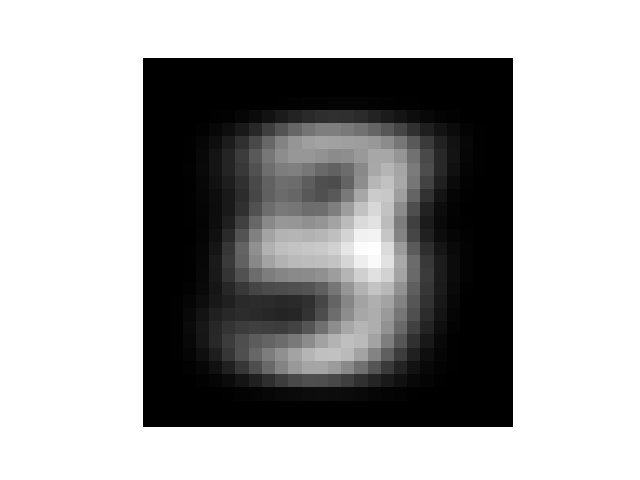
\includegraphics[width=.5\linewidth]{Pics/05_methodology/general.png}
    \end{subfigure}
    \caption{Scatter plot of the 2 loadings of the loading matrix $\bs{A}$ for the MNIST 3s and 4s respectively.}
    \label{fig:my_label}
\end{figure}
